\documentclass{standalone}\usepackage[]{graphicx}\usepackage[]{color}
%% maxwidth is the original width if it is less than linewidth
%% otherwise use linewidth (to make sure the graphics do not exceed the margin)
\makeatletter
\def\maxwidth{ %
  \ifdim\Gin@nat@width>\linewidth
    \linewidth
  \else
    \Gin@nat@width
  \fi
}
\makeatother

\definecolor{fgcolor}{rgb}{0.345, 0.345, 0.345}
\newcommand{\hlnum}[1]{\textcolor[rgb]{0.686,0.059,0.569}{#1}}%
\newcommand{\hlstr}[1]{\textcolor[rgb]{0.192,0.494,0.8}{#1}}%
\newcommand{\hlcom}[1]{\textcolor[rgb]{0.678,0.584,0.686}{\textit{#1}}}%
\newcommand{\hlopt}[1]{\textcolor[rgb]{0,0,0}{#1}}%
\newcommand{\hlstd}[1]{\textcolor[rgb]{0.345,0.345,0.345}{#1}}%
\newcommand{\hlkwa}[1]{\textcolor[rgb]{0.161,0.373,0.58}{\textbf{#1}}}%
\newcommand{\hlkwb}[1]{\textcolor[rgb]{0.69,0.353,0.396}{#1}}%
\newcommand{\hlkwc}[1]{\textcolor[rgb]{0.333,0.667,0.333}{#1}}%
\newcommand{\hlkwd}[1]{\textcolor[rgb]{0.737,0.353,0.396}{\textbf{#1}}}%

\usepackage{framed}
\makeatletter
\newenvironment{kframe}{%
 \def\at@end@of@kframe{}%
 \ifinner\ifhmode%
  \def\at@end@of@kframe{\end{minipage}}%
  \begin{minipage}{\columnwidth}%
 \fi\fi%
 \def\FrameCommand##1{\hskip\@totalleftmargin \hskip-\fboxsep
 \colorbox{shadecolor}{##1}\hskip-\fboxsep
     % There is no \\@totalrightmargin, so:
     \hskip-\linewidth \hskip-\@totalleftmargin \hskip\columnwidth}%
 \MakeFramed {\advance\hsize-\width
   \@totalleftmargin\z@ \linewidth\hsize
   \@setminipage}}%
 {\par\unskip\endMakeFramed%
 \at@end@of@kframe}
\makeatother

\definecolor{shadecolor}{rgb}{.97, .97, .97}
\definecolor{messagecolor}{rgb}{0, 0, 0}
\definecolor{warningcolor}{rgb}{1, 0, 1}
\definecolor{errorcolor}{rgb}{1, 0, 0}
\newenvironment{knitrout}{}{} % an empty environment to be redefined in TeX

\usepackage{alltt}
\usepackage{tikz}
\usepackage{pgfplots}
\usepackage{fontspec}
\usepackage{color}
\usetikzlibrary{decorations.text,intersections}
\pgfplotsset{compat=1.7}

\definecolor{nice_blue}{HTML}{377EB8}
\definecolor{nice_green}{HTML}{4DAF4A}
\definecolor{nice_purple}{HTML}{984EA3}
\definecolor{nice_red}{HTML}{E41A1C}
\definecolor{nice_orange}{HTML}{FF7F00}
\definecolor{nice_pink}{HTML}{FB9A99}

\pgfplotsset{
    simple graphs/.style={
        domain=0:12
        ,xmin=0
        ,xmax=12
        ,ymin=0
        ,ymax=12
        ,axis lines*=left
        ,xtick=\empty
        ,ytick=\empty
        ,every axis y label/.style={
            at={(axis description cs:0.09,.5)}
            ,rotate=90
            ,anchor=south},
        }
        ,every axis x label/.style={
            at={(axis description cs:0.5,-0.1)}
            ,anchor=south}
        }
\IfFileExists{upquote.sty}{\usepackage{upquote}}{}
\begin{document}
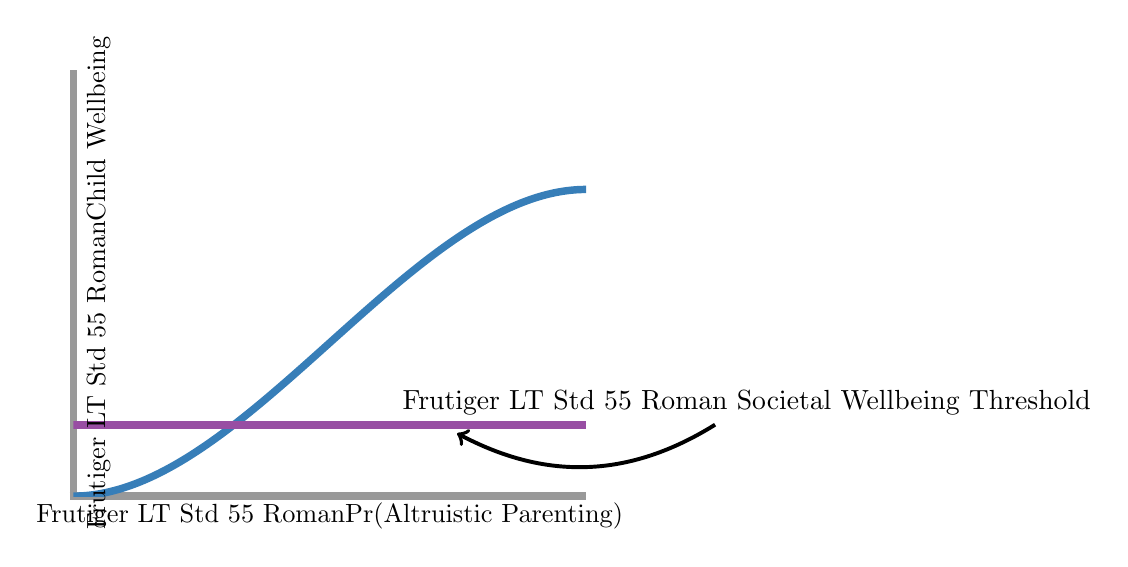
\begin{tikzpicture}[scale=0.95]

\def\myshift#1{\raisebox{2ex}}

\centering

\node (wbar) at (9,1.25) [draw=none,fill=none] {\fontspec{Frutiger LT Std 55 Roman} Societal Wellbeing Threshold};
\node (wbar_arrow_end) at (5,.9) [draw=none,fill=none] {};

\draw[->,bend left, line width=2.83464567*0.5pt]  (wbar) to node [auto] {} (wbar_arrow_end);

\begin{axis}[
    simple graphs,
    ytick=\empty,
    xtick=\empty,
    enlarge x limits=false,
    axis lines*=left,
    axis line style = {gray!80, line width=2.83464567pt,shorten <=-0.5\pgflinewidth},
    ymax=6,
    xmax=6,
    ylabel=\fontspec{Frutiger LT Std 55 Roman}Child Wellbeing, 
    xlabel=\fontspec{Frutiger LT Std 55 Roman}Pr(Altruistic Parenting)
]

\addplot[->
        ,nice_blue
        ,line width=2.83464567pt
        ,samples=1000] 
        {2*(.18*x^2 - .02*x^3)};
        
\addplot[nice_purple, line width=2.83464567pt] plot coordinates {
        (0,1)
        (6,1)};

\end{axis}

\end{tikzpicture}
\end{document}
